% 四張英文參考圖；分節正文已插入，本檔供複製到學姐專案。
% 每段含前導文字、figure、cite 與 label；已有同名標籤時不重複插入。
% 書目統一使用 thesis_references.bib。


% ==================================================
% 位置：Nav2 及定位來源介紹之後
% 2.4.1 英文參考圖：Navigation2 既有架構
% ==================================================
Nav2 的既有模組分工如\cref{fig:ref_nav2_architecture}所示，由任務協調層連結規劃、控制與恢復等服務。本研究使用其全域規劃與代價地圖功能，並以本文的預測控制與任務邏輯銜接後續導航及操作；圖中完整架構不等同於本研究各階段的實際啟用配置。

\begin{figure}[htbp]
    \centering
    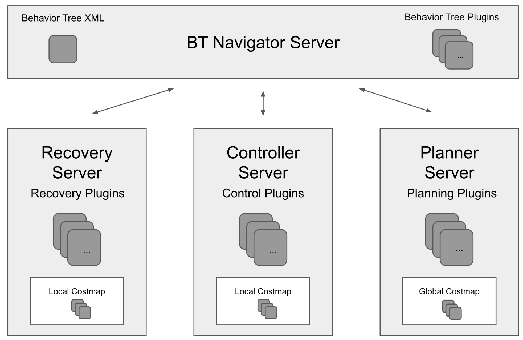
\includegraphics[width=0.86\textwidth]{figsrc/reference_figures/nav2_architecture_macenski2020.pdf}
    \caption{Navigation2 既有系統之模組分工（引自文獻\cite{macenski2020nav2}之圖~2）}
    \label{fig:ref_nav2_architecture}
\end{figure}

% ==================================================
% 位置：本小節末、3.1.2 之前
% 3.1.1 英文參考圖：旋轉群與角度參數
% ==================================================
旋轉群與角度參數的表示差異如\cref{fig:ref_rotation_representation}所示。角度在選定的主值區間邊界會出現包絡跳變，對應的旋轉矩陣則維持連續。此圖說明本研究採用幾何位姿表示的背景；底盤的全向運動模型仍依本研究輪系建立。

\begin{figure}[htbp]
    \centering
    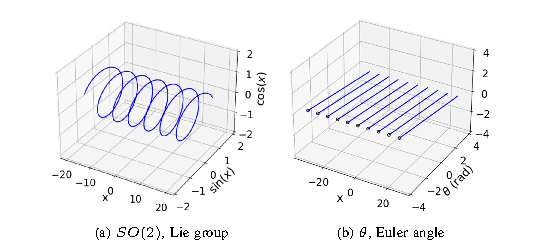
\includegraphics[width=0.95\textwidth]{figsrc/reference_figures/rotation_representation_tang2024.pdf}
    \caption{旋轉群與角度參數表示之比較（引自文獻\cite{tang2024gmpc}之圖~1）}
    \label{fig:ref_rotation_representation}
\end{figure}

% ==================================================
% 位置：等速度模型與符號說明之後
% 3.4.1 英文參考圖：卡爾曼濾波循環
% ==================================================
卡爾曼濾波的預測與量測更新流程如\cref{fig:ref_kalman_predict_update}所示。圖中的 $A$ 與 $H$ 分別對應本節的 $F_o(\Delta\tau)$ 與 $H_o$；障礙物運動未設定外部控制輸入，因此圖中的 $Bu$ 項取零。追蹤器先將位置與速度向前預測，再以新群集中心量測修正估計。

\begin{figure}[htbp]
    \centering
    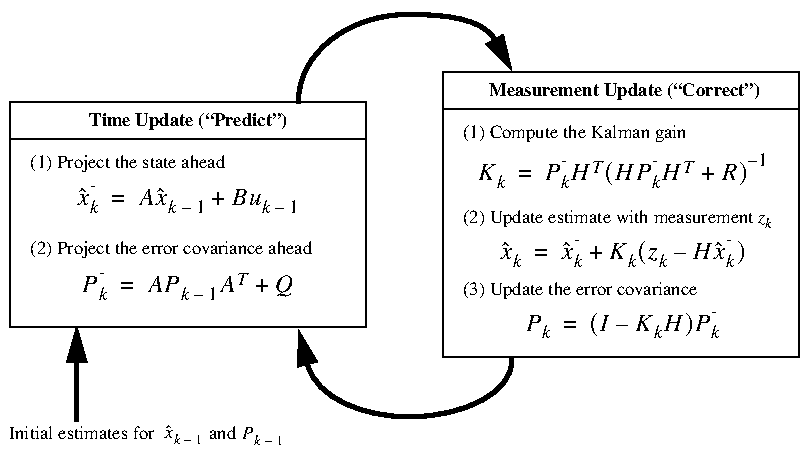
\includegraphics[width=0.98\textwidth]{figsrc/reference_figures/kalman_predict_update_welch2004.pdf}
    \caption{卡爾曼濾波之預測與量測更新流程（引自文獻\cite{welch2004kalman}之圖~1-2）}
    \label{fig:ref_kalman_predict_update}
\end{figure}

% ==================================================
% 位置：模型及訓練資料介紹之後
% 3.5.1 英文參考圖：Mask R-CNN 原理
% ==================================================
Mask R-CNN 的原始流程如\cref{fig:ref_mask_rcnn_framework}所示，對候選區域同時提供類別、外框與實例遮罩。此圖用於說明原方法概念；本研究採用前述 ResNet-50-FPN v2 實作，並將遮罩連結至深度幾何估測。

\begin{figure}[htbp]
    \centering
    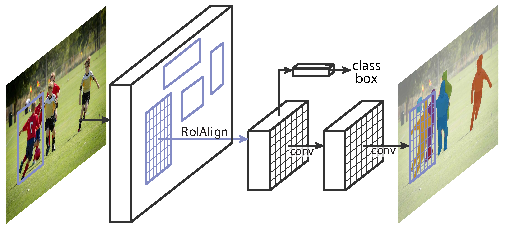
\includegraphics[width=0.95\textwidth]{figsrc/reference_figures/mask_rcnn_framework_he2017.pdf}
    \caption{Mask R-CNN 實例分割方法之原理示意（引自文獻\cite{he2017maskrcnn}之圖~1）}
    \label{fig:ref_mask_rcnn_framework}
\end{figure}
